\documentclass[a5paper,12pt]{article}
\usepackage[portuges]{babel}
\usepackage[latin1]{inputenc}
\usepackage{graphicx}
\usepackage[pdftex,plainpages=false,pdfpagelabels,
pagebackref,colorlinks=true,citecolor=blue,
linkcolor=black,urlcolor=blue,filecolor=blue,
bookmarksopen=true]{hyperref}
\usepackage{amsmath,amsfonts,mathrsfs,amssymb}
\usepackage{multicol}
\usepackage{fancyhdr}
\usepackage{makeidx} 
\usepackage[papersize={5.25in,7in},left=1cm,
right=1cm,top=2cm,bottom=2cm]{geometry}
\usepackage{fourier-orns}
\usepackage{mdframed,xcolor}
\usepackage{sectsty}
\usepackage{enumitem}

%%%%%%%%%%%%%%%%% Box Reflita %%%%%%%%%%%%%%%%%%%%%%%%%%%%
\newmdenv[shadow=false, shadowsize=2pt, linewidth=2pt,
frametitlerule=true, roundcorner=20pt,]{reflita}


%%%%%%%%%%%%%%%% comando regua %%%%%%%%%%%%%%%%%%%%%%%%%%%
\newcommand{\HRule}[1]{\rule{\linewidth}{#1}}


%%%%%%%%%%%%%%%%%%%%%%%%%%%%%%%%%%%%%%%%%%%%%%%%%%%%%%%%%%%
\numberwithin{equation}{section}
\setlength{\parskip}{2pt}
\sectionfont{\large}
\renewcommand{\baselinestretch}{1.2}
\pagestyle{fancy}
\fancyfoot[LO,L]{osvald23@gmail.com}
\fancyfoot[RO,R]{O.L.S., Pereira}


%%%%%%%%%%%%%%%%%%%%%%%%%%%%%%%%%%%%%%%%%%%%%%%%%%%%%%%%%%%
%\setlength{\textheight}{240mm}
%\setlength{\textwidth}{145mm}
\setlength{\headheight}{15.8pt}
%\renewcommand{\headrulewidth}{0.5pt}
\renewcommand{\footrulewidth}{0.5pt}
%\renewcommand{\baselinestretch}{1.3}


\makeindex
\begin{document}

\begin{titlepage} 
\begin{center}
\normalsize \textsc{Cole��o Matem�tica Divertida} 	%Subtitle
		 	\\[1.0cm]								% 2cm spacing
			\HRule{0.5pt} \\ [0.5cm]			% Upper rule
			
			{\LARGE \textbf{Teoria de Grafos}}% Title
			
			\HRule{0.5pt} \\ [0.5cm]		% Lower rule + 0.5cm spacing
\end{center}

\begin{figure}[!ht]
 \centering
 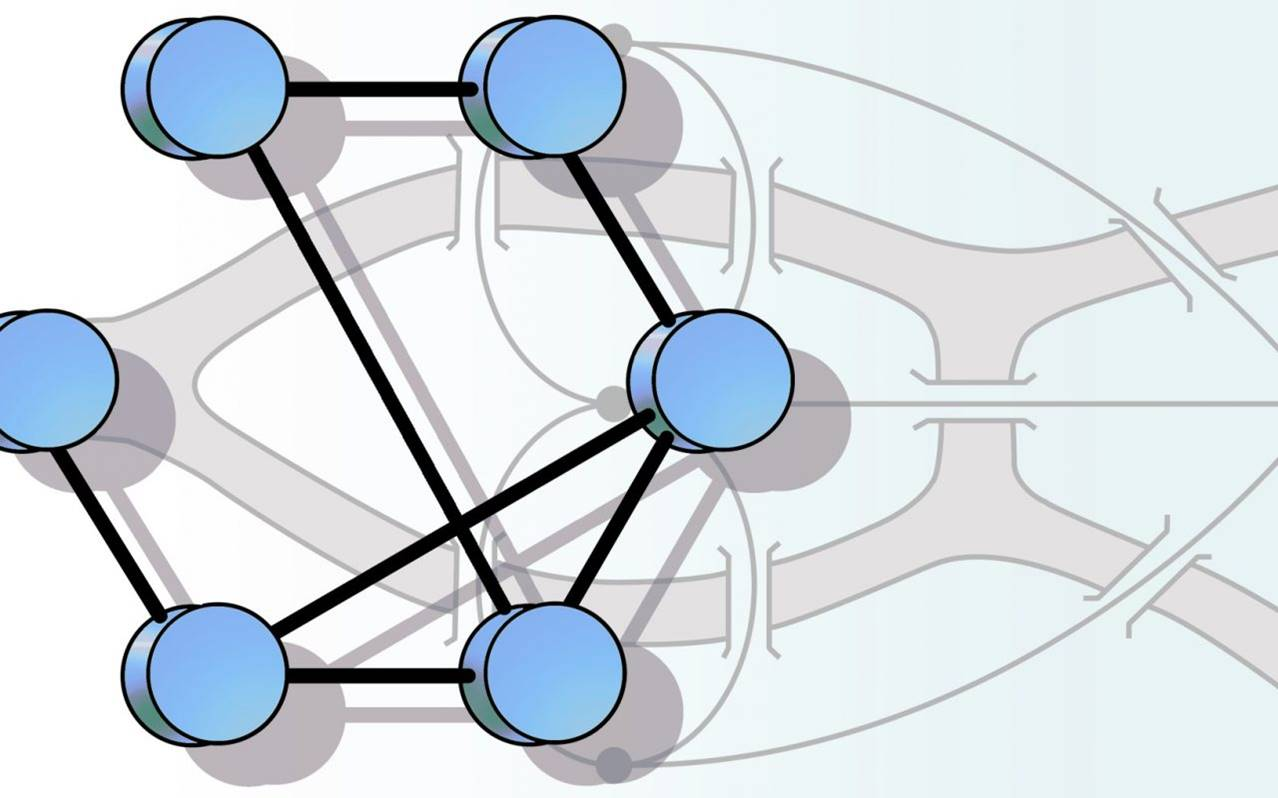
\includegraphics[scale=0.4]{cover.jpg}
 %\caption{}
 \label{cover}
\end{figure}

%\vspace{0.5cm}

Autor: Osvaldo Luiz dos Santos Pereira

e-mail: \texttt{osvald23@gmail.com} 
\end{titlepage} 


\tableofcontents
%\listoffigures

\section*{Pref�cio}
\addcontentsline{toc}{section}{Pref�cio}

Neste breve livro, tive como objetivo apresentar de uma 
forma divertida, um tema de pesquisa em matem�tica, 
a Teoria de Grafos, para crian�as em idade de ensino 
fundamental (de 8 a 14 anos), mas que tamb�m possa 
ser aproveitado por jovens adultos, e adultos que tenham 
curiosidade pela matem�tica. O livro trata de forma bem 
b�sica as defini��es prim�rias do assunto. Em nenhum 
momento tem a pretens�o de ser um livro t�cnico, mas 
sim uma ponte entre o desconhecimento, e a vontade de 
aprender mais sobre algo interessante. O livro aborda a 
defini��o de grafos, v�rtices, arestas, caracter�stica 
de Euler, s�lidos 3D, e n�mero crom�tico. 

O ensino da matem�tica pode ser um agente transformador, 
aumentar a auto estima, e transformar vidas, desenvolvendo 
habilidades cognitivas muito importantes. Qualquer sociedade 
deveria priorizar o ensino de matem�tica e ci�ncias para 
crian�as e jovens, se deseja ter uma na��o desenvolvida 
no futuro. Espero que com este despretensioso livro, 
possa somar, mesmo que seja um pouquinho.


%%%%%%%%%%%%%%%%%%%%%%%%%%%%%%%%%%%%%%%%%%%%%%%%%%%%%%%%%%%
\newpage\section*{Agradecimentos}
\addcontentsline{toc}{section}{Agradecimentos}

Tenho muitas pessoas queridas em minha vida, amigos, fam�lia 
e gostaria de poder agradecer a todos, listando neste espa�o, 
mas isso seria uma tarefa improv�vel de ser cumprida. 
Portanto se voc� estiver lendo este livro, o motivo � o meu 
agradecimento! Mas n�o poderia deixar de mencionar a minha 
esposa Adriana Jardim Arias Pereira, a quem devo tudo que 
conquistei at� hoje, pelo seu apoio, paix�o, amor, respeito, 
e companheirismo. � minha terapeuta Simone que foi a pessoa 
que mais me apoiou neste projeto, e me ajudou a materializar 
e finalizar este empreendimento pessoal. � ela sou muito grato. 
E tamb�m gostaria de agradecer minha amiga (e chefe) Ticiana
Sales Leon, por ter me apoiado em momentos dif�ceis e complexos, 
e por ter acreditado em mim. Logicamente n�o poderia deixar 
de agradecer meus pais Osvaldo Monteiro Pereira e Lilian Fran�a
dos Santos Monteiro Periera, meus irm�os Caio Cezar dos Santos 
Pereira, e Paulo Fernando dos Santos Pereira, minha madrinha 
Terezinha Fran�a, e minha tia Eliana. Eles sempre me deram 
apoio incondicional. Muito obrigado!


%%%%%%%%%%%%%%%%%%%%%%%%%%%%%%%%%%%%%%%%%%%%%%%%%%%%%%%%%%%
\newpage\section*{In Memorian}
\addcontentsline{toc}{section}{In Memorian}
Milton Eleres dos Santos, Socorro Fran�a dos Santos, 
Osvaldo Monteiro Pereira, Paulo Zacca, Vanda, Rodrigo, 
Mario, Heitor.
\section{O Que S�o Grafos?}


%%%%%%%%%%%%%%%%%%%%%%%%%%%%%%%%%%%%%%%%%%%%%%%%%%%%%%%%%%%
\subsection{Introdu��o}

� um ramo da matem�tica que consiste em explicar atrav�s de
modelos e fun��es matem�ticas, os tipos de rela��es entre 
um grupo de objetos. Por exemplo, designar a melhor rota de 
visita entre cidades vizinhas, a conex�o entre neur�nios, 
configura��o de circuitos eletr�nicos, etc. Possui vasta 
aplica��o em �reas como f�sica, neuroci�ncia, computa��o, 
lingu�stica, ci�ncias sociais, e tamb�m no desenvolvimento 
e aperfei�oamento de redes sociais, etc. 

Um exemplo de aplica��o em redes sociais seria o Facebook, 
e seus algoritmos de sugest�o do feed de not�cias, de 
sugest�o de amigos, etc. 

A teoria de grafos teve seu in�cio em um artigo publicado 
em 1736, por Leonhard Euler, no qual resolve o famoso 
problema conhedico por `s sete pontes de Konigsberg'. 
A literatura sobre o assunto � muito vasta, e em geral 
muito t�cnica. Este livro n�o tem como pretens�o substituir 
esse tipo de literatura. O escopo deste livro � fazer um 
breve passeio nos primeiros princ�pios sobre este ramo 
fascinante da matem�tica.


%%%%%%%%%%%%%%%%%%%%%%%%%%%%%%%%%%%%%%%%%%%%%%%%%%%%%%%%%%%
\newpage\subsection{Definindo Grafos}

Nesta parte do livro vamos introduzir a defini��o de grafos, 
e apresentar algumas defini��es. Definiremos o que s�o 
v�rtices, arestas, e apresentaremos a caracter�stica de 
Euler.

Um grafo � uma cole��o de v�rtices (V) conectados por arestas 
(A), formando regi�es (R) bem definidas e limitadas.

\index{aresta}
\index{v�rtice}
\index{regi�o}

\begin{figure}[!ht]
 \centering
 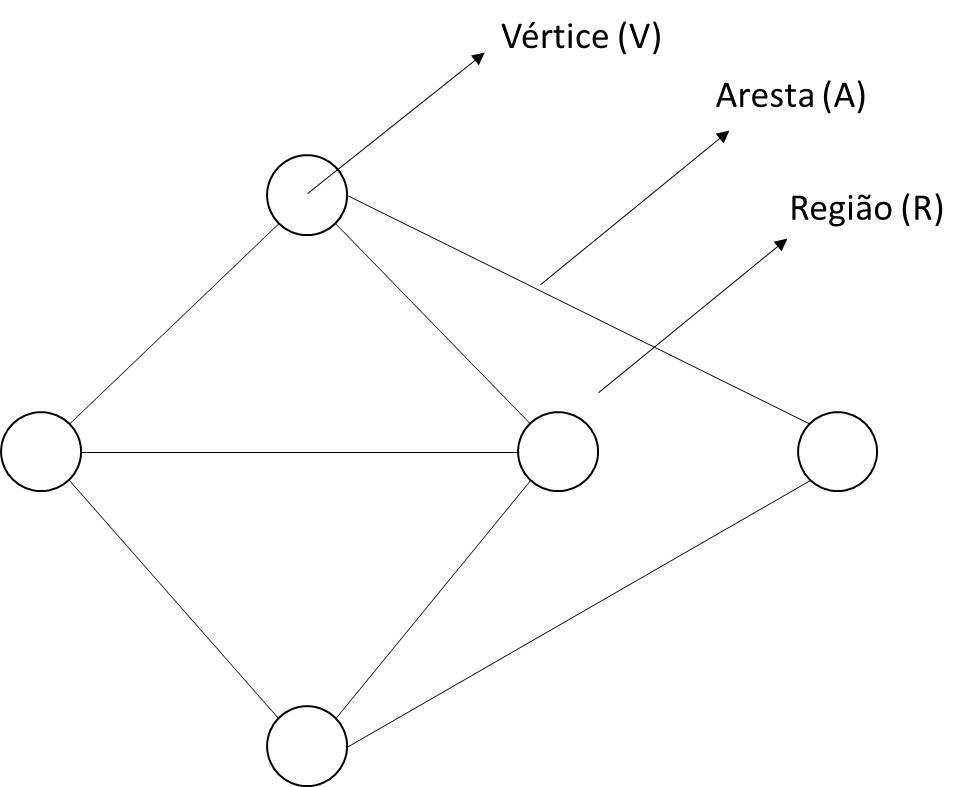
\includegraphics[scale=0.45]{1.jpg}
 \caption{Imagem de um grafo que possui 5 v�rtices (V), 
 7 arestas (A), e 4 regi�es (R).}
 \label{1}
\end{figure}


%%%%%%%%%%%%%%%%%%%%%%%%%%%%%%%%%%%%%%%%%%%%%%%%%%%%%%%%%%%
\newpage

O matem�tico Leonhard Euler descobriu que ao somar o n�mero
de v�rtices ao n�mero de regi�es, e subtrair o n�mero de 
arestas, algo m�gico acontecia! O n�mero 
%
\[
V - A + R,
\]
%
hoje � conhecido como \textbf{\emph{Caracter�stica de 
Euler}}.

\begin{figure}[!ht]
 \centering
 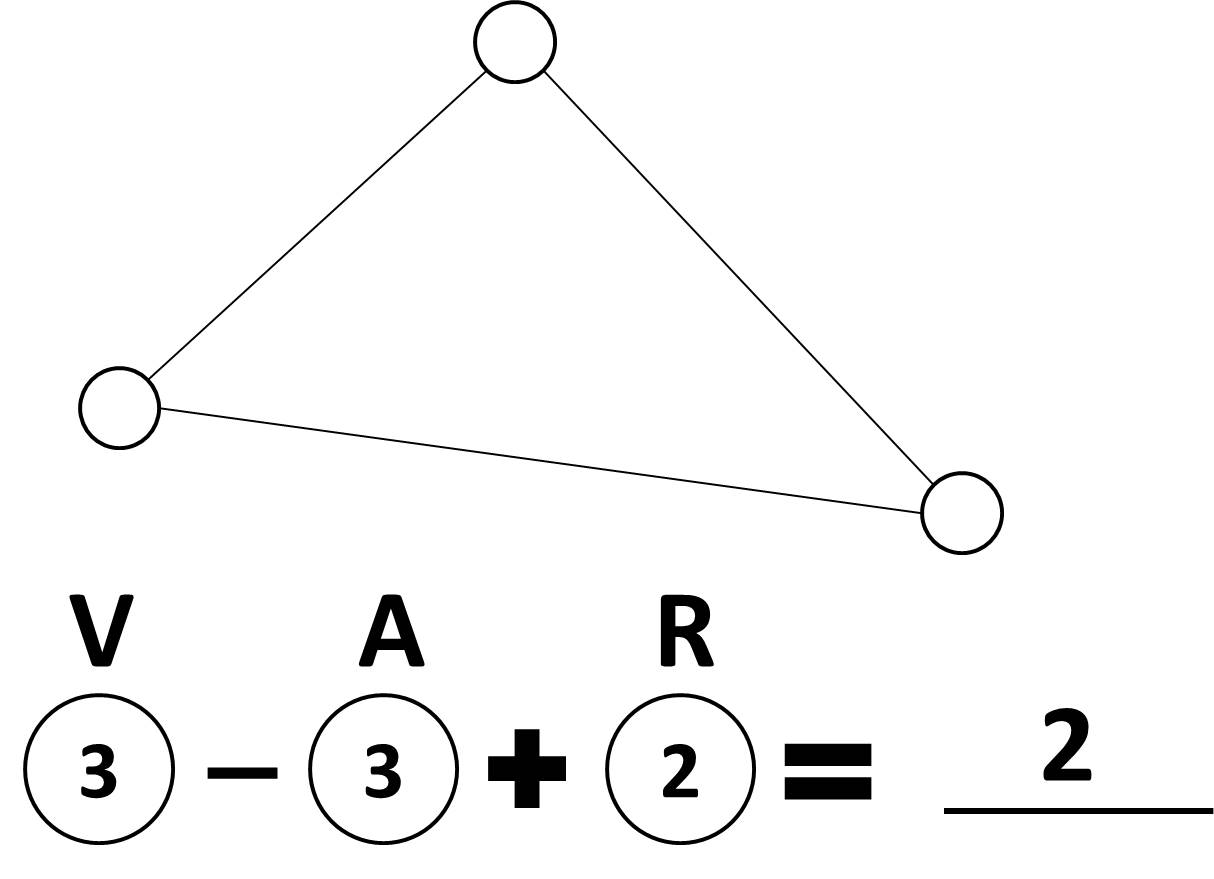
\includegraphics[scale=0.45]{2.jpg}
 \caption{Imagem de um grafo que possui V v�rtices (V), 
 A arestas (A), e R regi�es (R).}
 \label{2}
\end{figure}


%%%%%%%%%%%%%%%%%%%%%%%%%%%%%%%%%%%%%%%%%%%%%%%%%%%%%%%%%%%
\newpage

\begin{figure}[!ht]
 \centering
 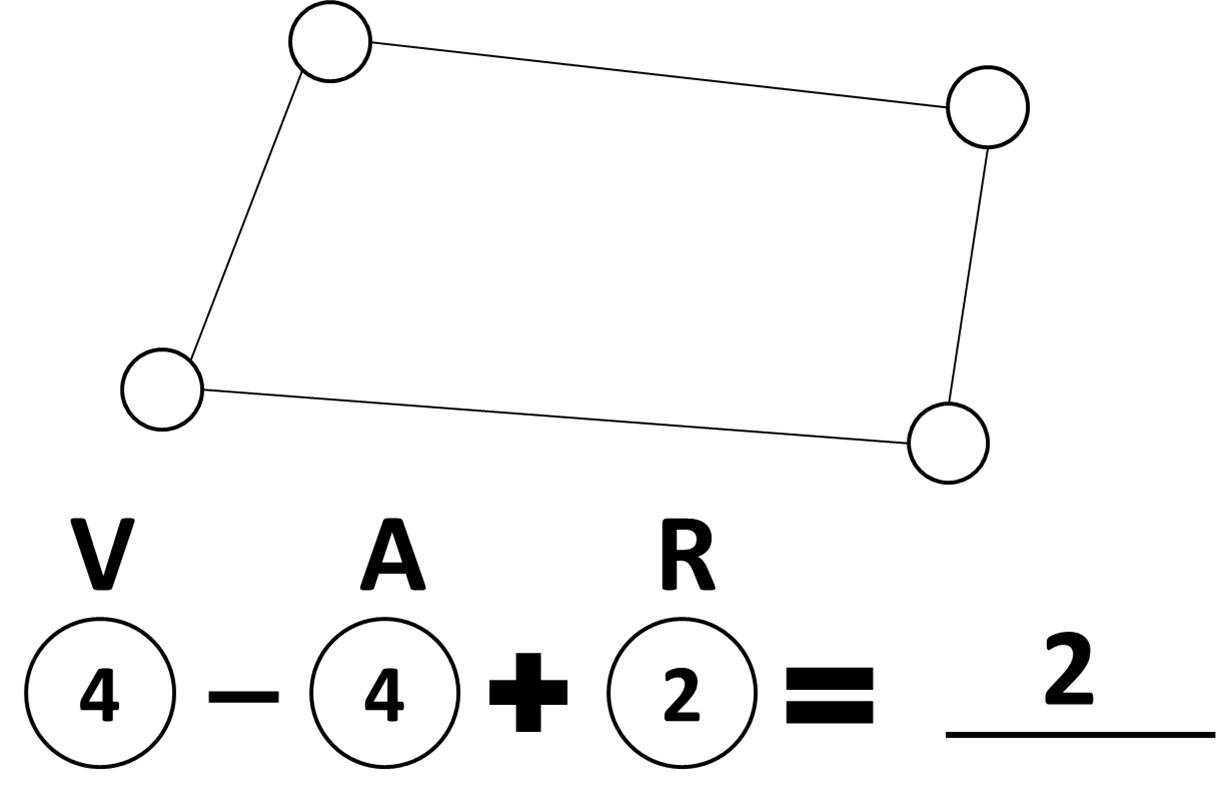
\includegraphics[scale=0.5]{3.jpg}
 \caption{Imagem de um grafo que possui V v�rtices (V), 
 A arestas (A), e R regi�es (R).}
 \label{3}
\end{figure}


%%%%%%%%%%%%%%%%%%%%%%%%%%%%%%%%%%%%%%%%%%%%%%%%%%%%%%%%%%%
\newpage


\begin{figure}[!ht]
 \centering
 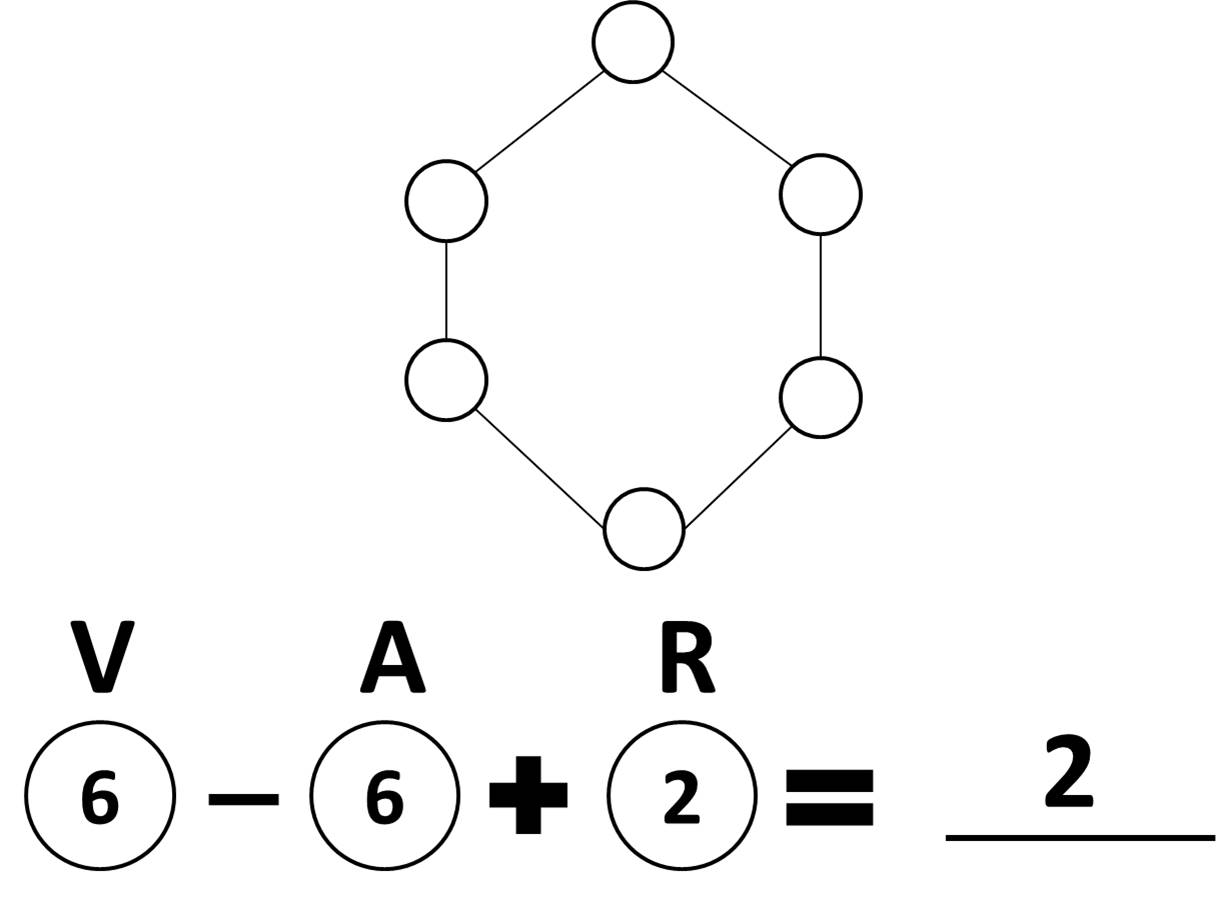
\includegraphics[scale=0.5]{4.jpg}
 \caption{Imagem de um grafo que possui V v�rtices (V), 
 A arestas (A), e R regi�es (R).}
 \label{4}
\end{figure}


%%%%%%%%%%%%%%%%%%%%%%%%%%%%%%%%%%%%%%%%%%%%%%%%%%%%%%%%%%%
\newpage

\begin{figure}[!ht]
 \centering
 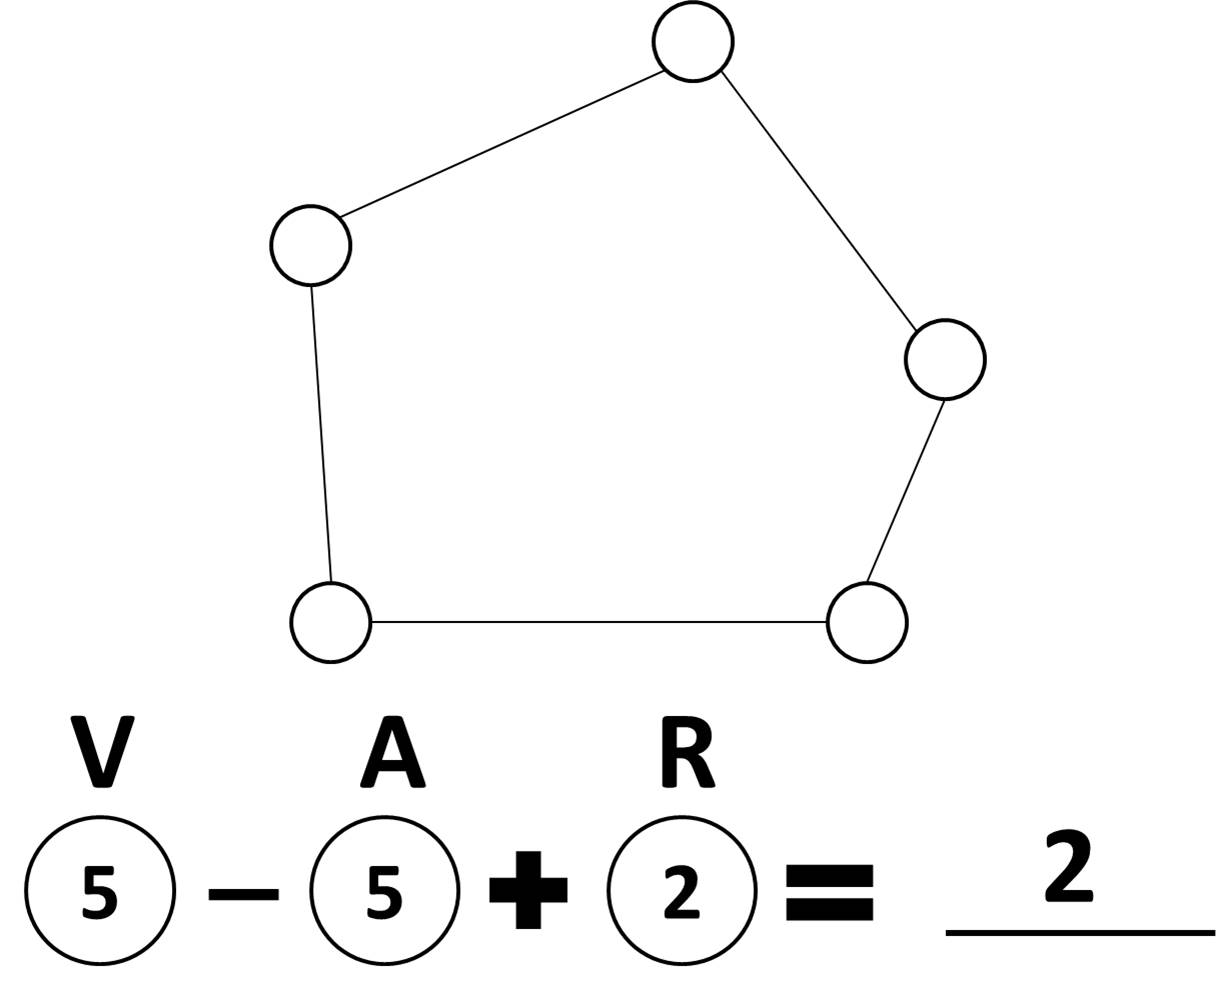
\includegraphics[scale=0.5]{5.jpg}
 \caption{Imagem de um grafo que possui V v�rtices (V), 
 A arestas (A), e R regi�es (R).}
 \label{5}
\end{figure}


%%%%%%%%%%%%%%%%%%%%%%%%%%%%%%%%%%%%%%%%%%%%%%%%%%%%%%%%%%%
\newpage

\begin{figure}[!ht]
 \centering
 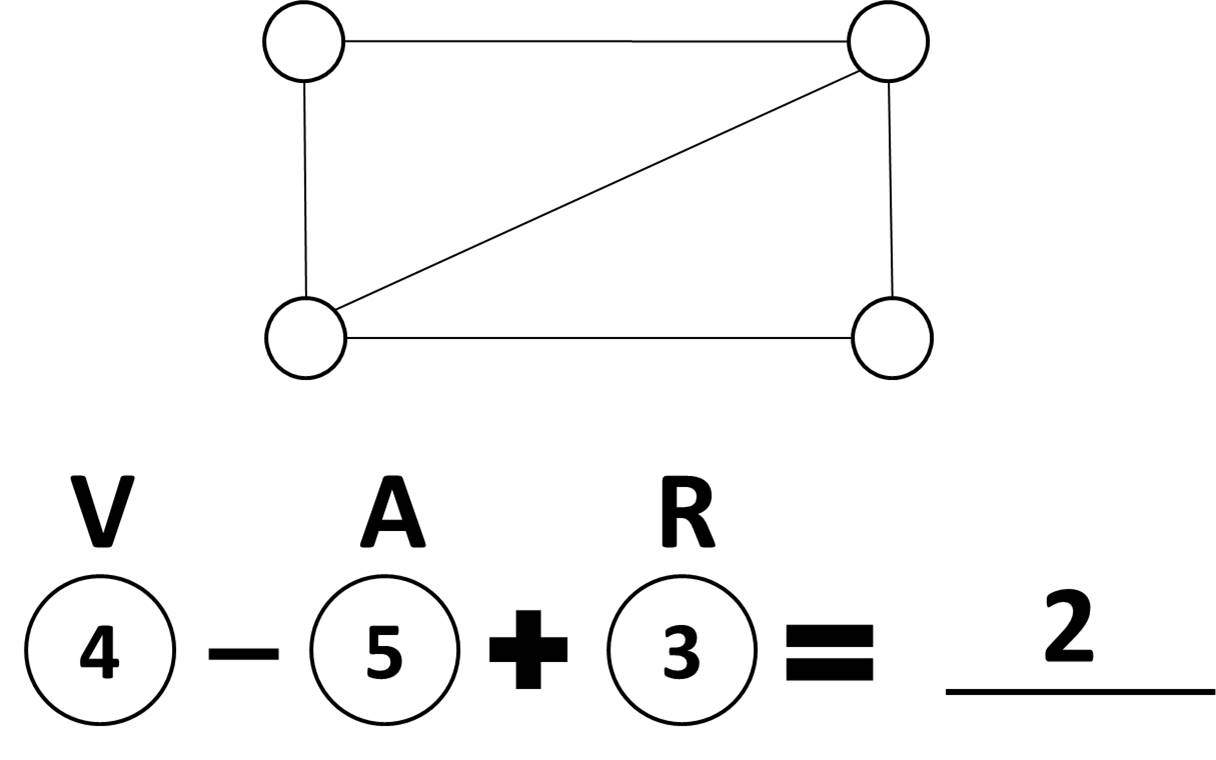
\includegraphics[scale=0.5]{6.jpg}
 \caption{Imagem de um grafo que possui V v�rtices (V), 
 A arestas (A), e R regi�es (R).}
 \label{6}
\end{figure}


%%%%%%%%%%%%%%%%%%%%%%%%%%%%%%%%%%%%%%%%%%%%%%%%%%%%%%%%%%%
\newpage

\begin{figure}[!ht]
 \centering
 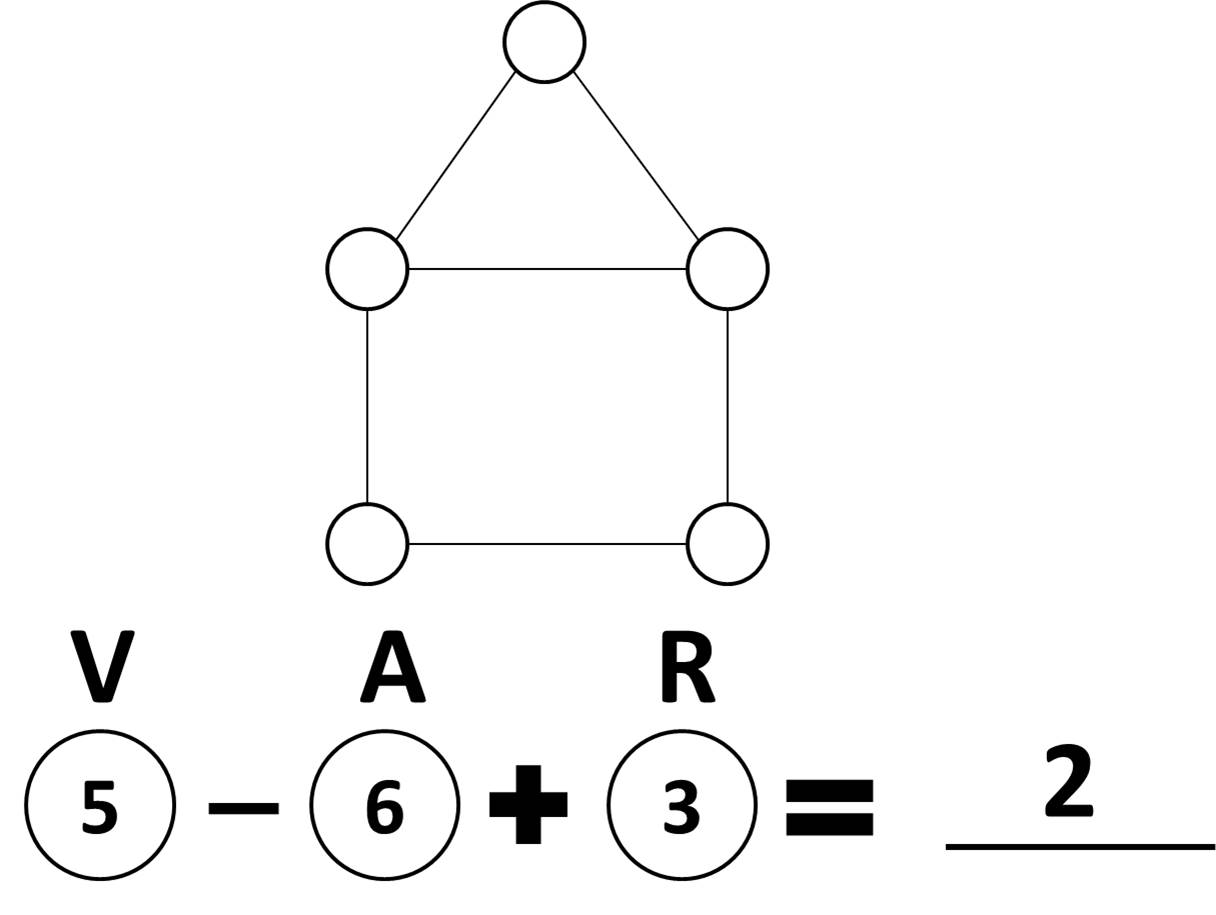
\includegraphics[scale=0.5]{7.jpg}
 \caption{Imagem de um grafo que possui V v�rtices (V), 
 A arestas (A), e R regi�es (R).}
 \label{7}
\end{figure}



%%%%%%%%%%%%%%%%%%%%%%%%%%%%%%%%%%%%%%%%%%%%%%%%%%%%%%%%%%%
\newpage

\begin{figure}[!ht]
 \centering
 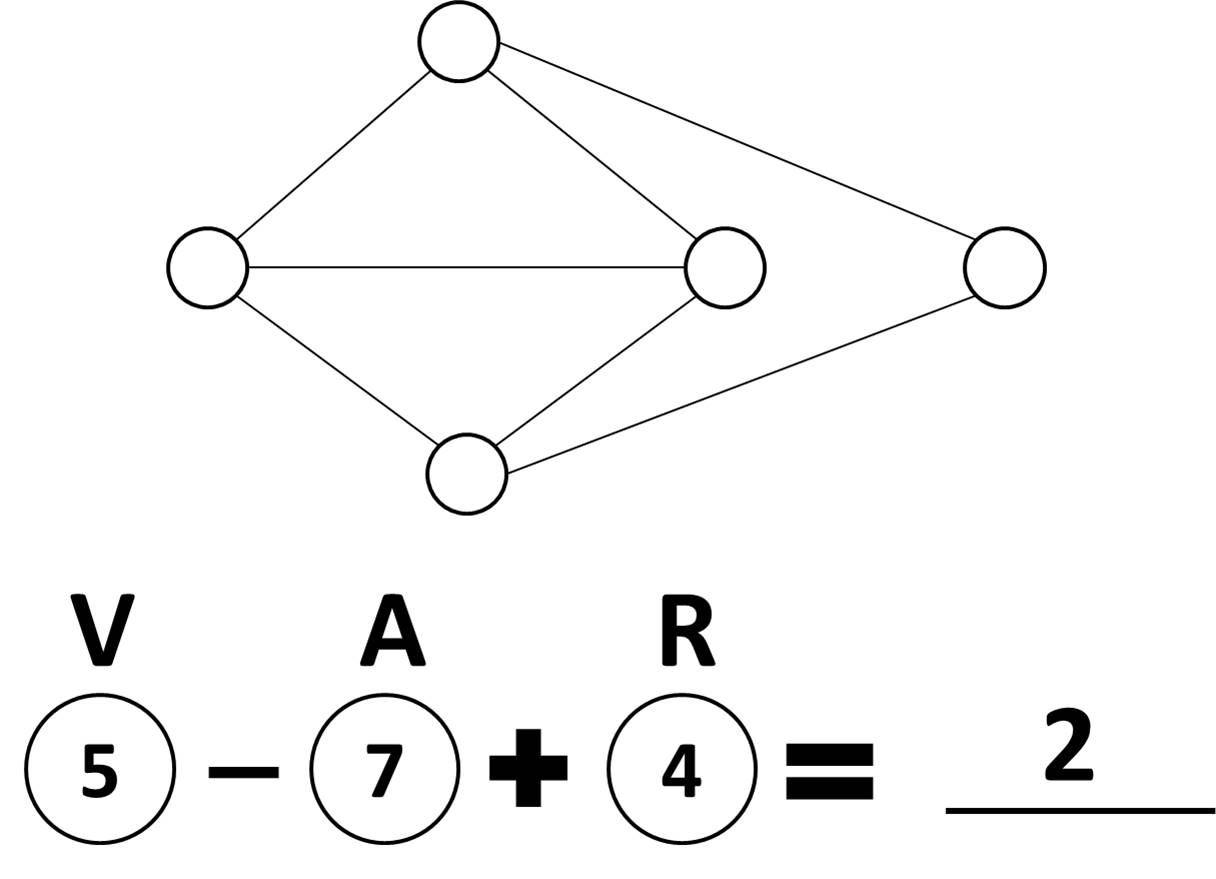
\includegraphics[scale=0.5]{8.jpg}
 \caption{Imagem de um grafo que possui V v�rtices (V), 
 A arestas (A), e R regi�es (R).}
 \label{8}
\end{figure}


%%%%%%%%%%%%%%%%%%%%%%%%%%%%%%%%%%%%%%%%%%%%%%%%%%%%%%%%%%%
\newpage

\begin{figure}[!ht]
 \centering
 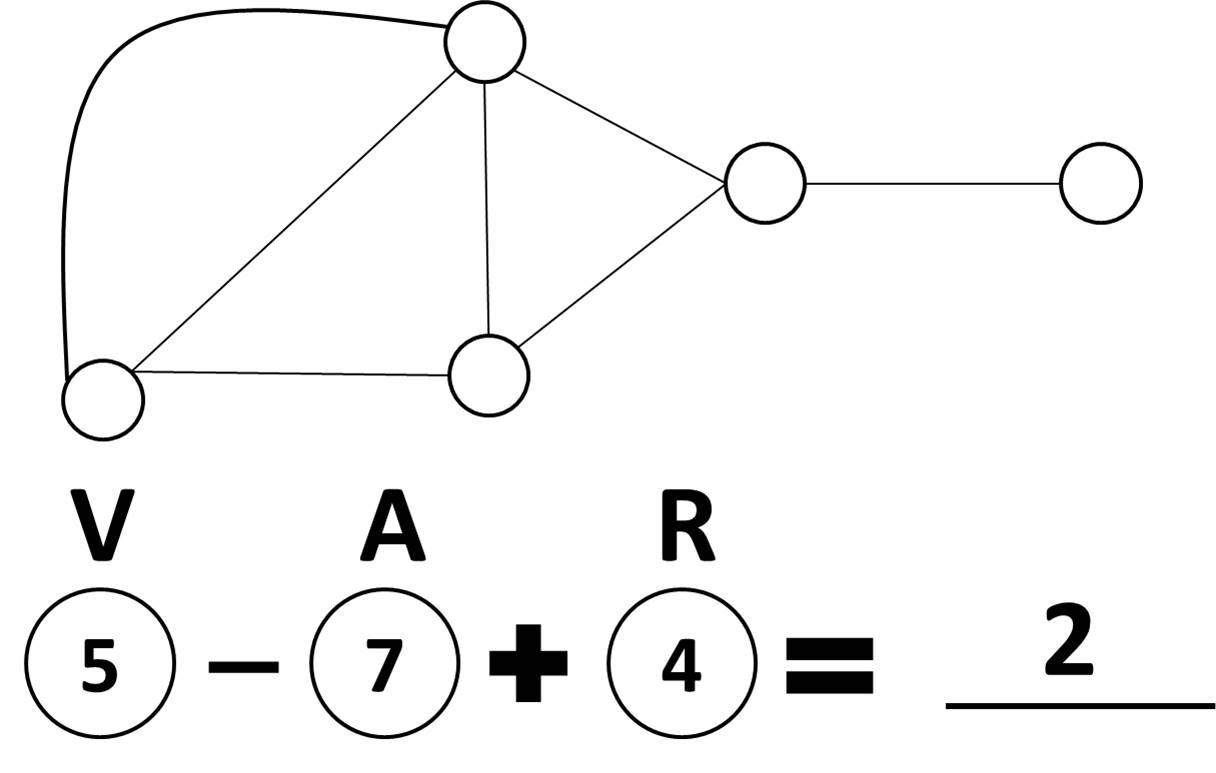
\includegraphics[scale=0.5]{9.jpg}
 \caption{Imagem de um grafo que possui V v�rtices (V), 
 A arestas (A), e R regi�es (R).}
 \label{9}
\end{figure}


%%%%%%%%%%%%%%%%%%%%%%%%%%%%%%%%%%%%%%%%%%%%%%%%%%%%%%%%%%%
\newpage

\begin{figure}[!ht]
 \centering
 
\includegraphics[scale=0.5]{10.jpg}
 \caption{Imagem de um grafo que possui V v�rtices (V), 
 A arestas (A), e R regi�es (R).}
 \label{10}
\end{figure}


%%%%%%%%%%%%%%%%%%%%%%%%%%%%%%%%%%%%%%%%%%%%%%%%%%%%%%%%%%%
\newpage

O que aconteceu com este grafo? A caracter�stica de Euler
n�o � mais igual a 2! A resposta � bem direta. Este grafo 
n�o respeita uma propriedade chamada \textit{conexidade}, 
ou seja, � dito ser um \textit{grafo n�o conexo}.

\index{conexidade} 
\index{grafo n�o conexo}

\begin{figure}[!ht]
 \centering
 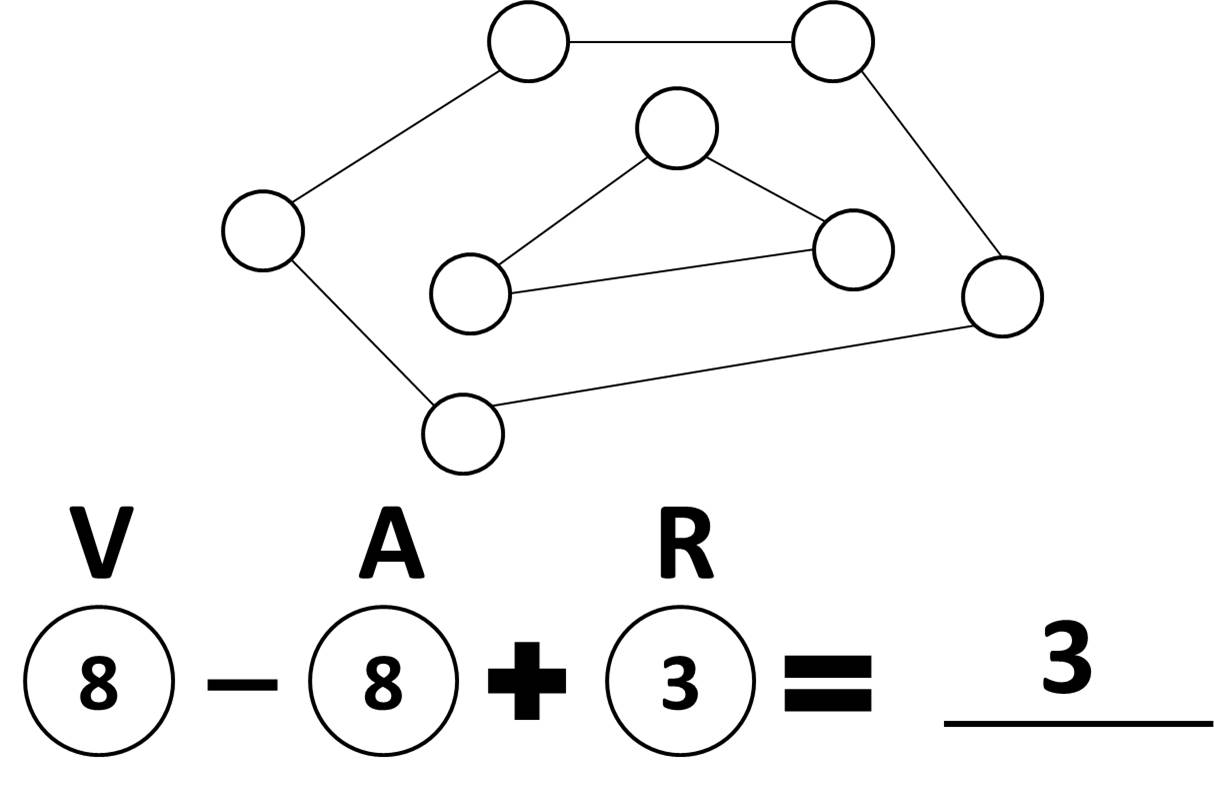
\includegraphics[scale=0.5]{11.jpg}
 \caption{Imagem de um grafo que possui V v�rtices (V), 
 A arestas (A), e R regi�es (R).}
 \label{11}
\end{figure}

{\Large Podemos `consertar' esse grafo?}


%%%%%%%%%%%%%%%%%%%%%%%%%%%%%%%%%%%%%%%%%%%%%%%%%%%%%%%%%%%
\newpage

{\Large Sim, podemos!} 

Basta acrescentarmos um v�rtice conectando a parte interior 
com a parte exterior como mostra a figura abaixo.


\begin{figure}[!ht]
 \centering
 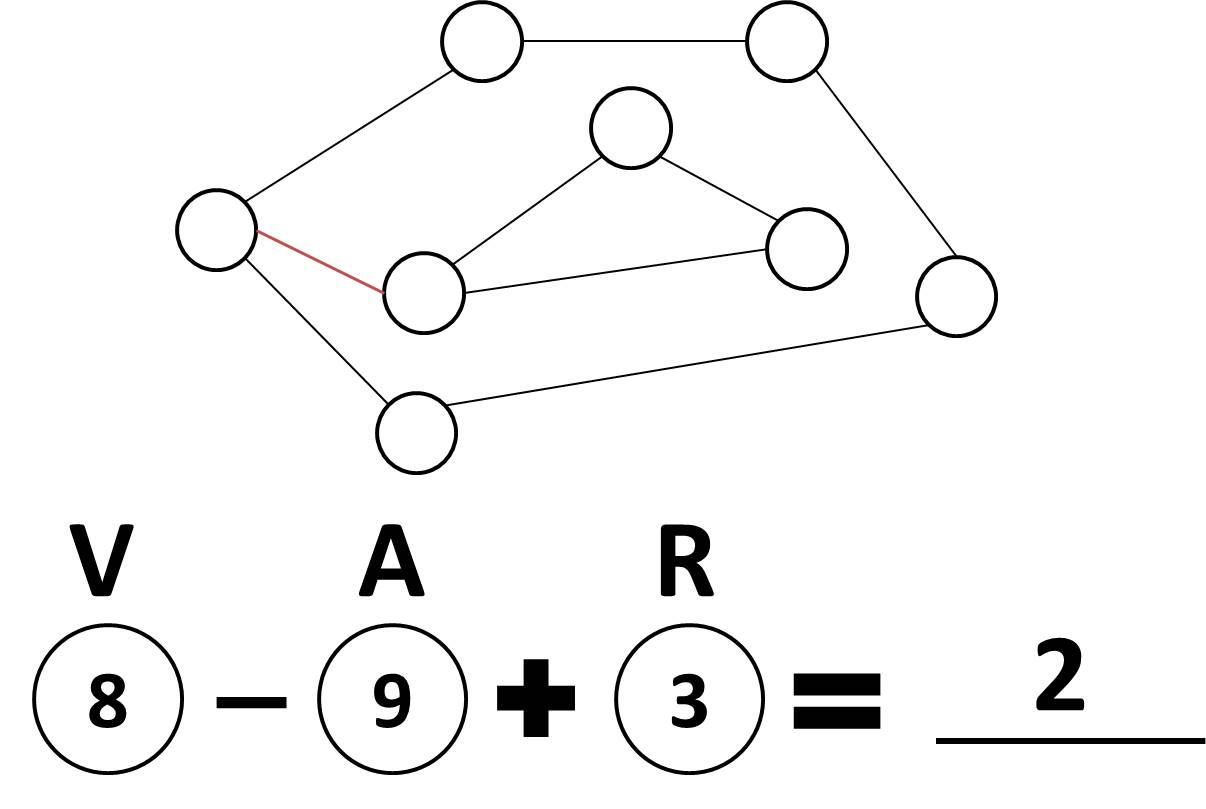
\includegraphics[scale=0.5]{12.jpg}
 \caption{Imagem de um grafo que possui V v�rtices (V), 
 A arestas (A), e R regi�es (R).}
 \label{12}
\end{figure}

%%%%%%%%%%%%%%%%%%%%%%%%%%%%%%%%%%%%%%%%%%%%%%%%%%%%%%%%%%%
\newpage\subsection{Gr�fico Conexo}

Um grafo � dito conexo se for poss�vel estabelecer um 
caminho de qualquer v�rtice para qualquer outro v�rtice.

Podemos definir o grau de conexidade de um gr�fico (k), 
bastando remover um n�mero k-1 de v�rtices, e perceber se 
o grafo continua sendo conexo. 

Para o nosso exemplo, o grau de conexidade � igual a 0. 
Pois se retirarmos uma aresta, o grafo deixa de ser 
conexo!

\index{conexo}
\index{conexidade}



%%%%%%%%%%%%%%%%%%%%%%%%%%%%%%%%%%%%%%%%%%%%%%%%%%%%%%%%%%%
\newpage\subsection{Gr�fico Planar}

� aquele grafo que pode ser representado em um plano sem 
qualquer interse��o entre arestas. At� agora todos os 
exemplos de grafos que estudamos s�o planares. Que tal
vermos um exemplo de gr�fico n�o planar?

\begin{figure}[!ht]
 \centering
 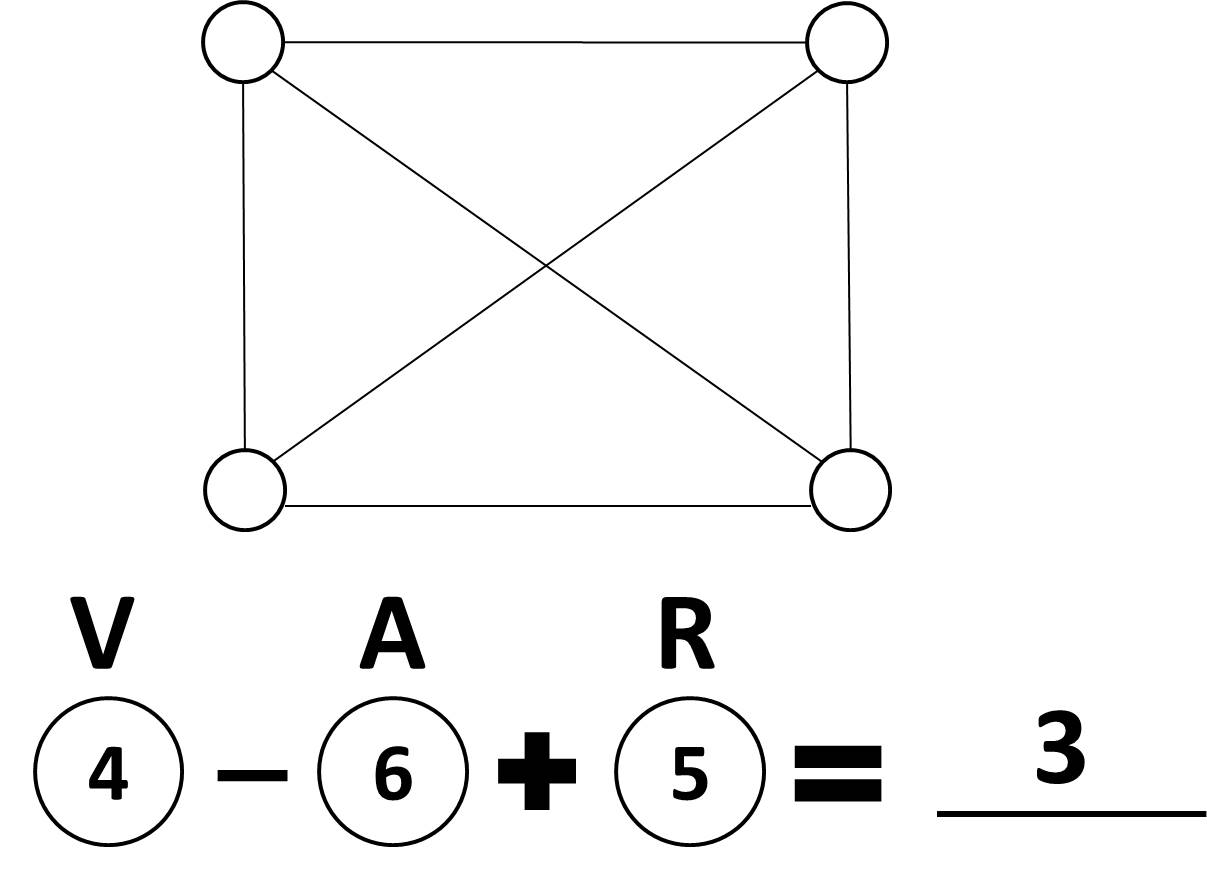
\includegraphics[scale=0.5]{13.jpg}
 \caption{Imagem de um grafo que possui V v�rtices (V), 
 A arestas (A), e R regi�es (R).}
 \label{13}
\end{figure}

\index{planar}
\section{S�lidos em 3D}
\section{Colorindo Grafos}

\begin{thebibliography}{}

\bibitem{Fulano}
Fulano de Tal, Livro, RJ, 2017. 
\end{thebibliography}
  
\printindex
\end{document}